\section{UAV-Bottle Dataset}
\label{sec:dataset}


%% 1. 图片收集方式
\subsection{Dataset collection}
\label{ssec:image_collection}

In the former section, we analyzed the challenges that bottle detection may encounter in the UAV perspective.
\begin{itemize}
	%% 1. 尺度问题
	\item The size of the bottles is very small and their scales change very much in UAV images. For solving this problem, we collect images at different flight altitudes.
	
	%% 2. 背景复杂
	\item In UAV images, the backgrounds of the bottles are very complex. In order to increase the diversity of dataset, we classify the possible scenes and divide them into eight scenes. Eight scenes are illustrated in Fig.\ref{fig:dataset-original-image}. and Fig.\ref{fig:dataset-cut-image}. In Fig.\ref{fig:dataset-original-image}., we show eight full images of eight scenes whose sizes are $ 5472\times 3078 $. In Fig.\ref{fig:dataset-cut-image}., we show the segmented images of eight scenes, each scene contains three images whose sizes are $ 342 \times 342 $.
	
	%% 3. 瓶子旋转
	\item The bottles in UAV images often appear with arbitrary orientations. We find the orientation of bottles will affect the robustness of the trained model, so we annotate images by using the oriented bounding box.
	
	%% 4. 瓶子透明
	\item The plastic bottles are usually transparent, so the background can be seen through the bottle, increasing the difficulty of detection. Our dataset includes a lot of examples of  transparent bottles, so we can use this large dataset to train a robust model.
\end{itemize}
%\begin{enumerate}[1. ]
%	%% 1. 尺度问题
%	\item The size of the bottles is very small, their sizes are generally less than $ 50\times 50 $ pixels. At the same time, due to the different altitudes of the UAV, their scales change very much. For solving this problem, we collect images at different flight altitudes of the UAV.
%	
%	%% 2. 背景复杂
%	\item In UAV images, the backgrounds of the bottles are very complex, resulting in poor performance of the general algorithm. In order to increase the diversity of dataset, we classify the possible scenes and divide them into eight scenes, each with a different number of images. Eight scenes are illustrated in Fig.\ref{fig:dataset-original-image} and Fig.\ref{fig:dataset-cut-image}. In Fig.\ref{fig:dataset-original-image}, we show eight full images of eight scenes whose sizes are $ 5472\times 3078 $. In Fig.\ref{fig:dataset-cut-image}, we show the segmented images of eight scenes, each scene contains three images whose size are $ 342 \times 342 $.
%	
%	%% 3. 瓶子旋转
%	\item In contrast to conventional object detection datasets, the bottles in UAV images often appear with arbitrary orientations, depending on the perspective of the UAV camera. We find the orientation of bottles will affect the robustness of the trained model, so we annotated images by using the oriented bounding box.
%	
%	%% 4. 瓶子透明
%	\item The plastic bottles as rubbish are usually transparent, so the background can be seen from the bottle, increasing the difficulty of detection. Our dataset includes a lot of transparent bottles, so we can use this large dataset to train a robust model.
%\end{enumerate}



The UAV platform used in this work is DJI Phantom 4 quadcopter integrated with a 3-axis stabilized gimbal.

Images are collected by a camera mounted on the quadcopter. The resolution of the captured images are $ 5472\times 3078 $. For dataset collection, we follow three key suggestions: (1) collecting images with bottles of a wide range of scale and aspect ratios; (2) collecting images with bottles of different background scenes; (3) collecting images with bottles of different orientations; (4) using as many types of bottles as possible. 


To collect images covering bottles of a wide range of scales and aspect ratios, images at different flight altitudes ranging from $ 10m $ to $ 30m $ are collected. Eight background scenes are chosen and annotated in our UAV-BD, including \textit{Bush forest land}, \textit{Waste land}, \textit{Step}, \textit{Forest land}, \textit{Flat ground}, \textit{Plastic stadium}, \textit{Sand land} and \textit{Grassland}. In this work, UAV images are collected from two periods. For each period, images are collected by using different bottles and different flight altitudes. The background scenes are selected according to whether a kind of scene is common and its value for real-world applications\cite{DOTA}.

\begin{figure}
	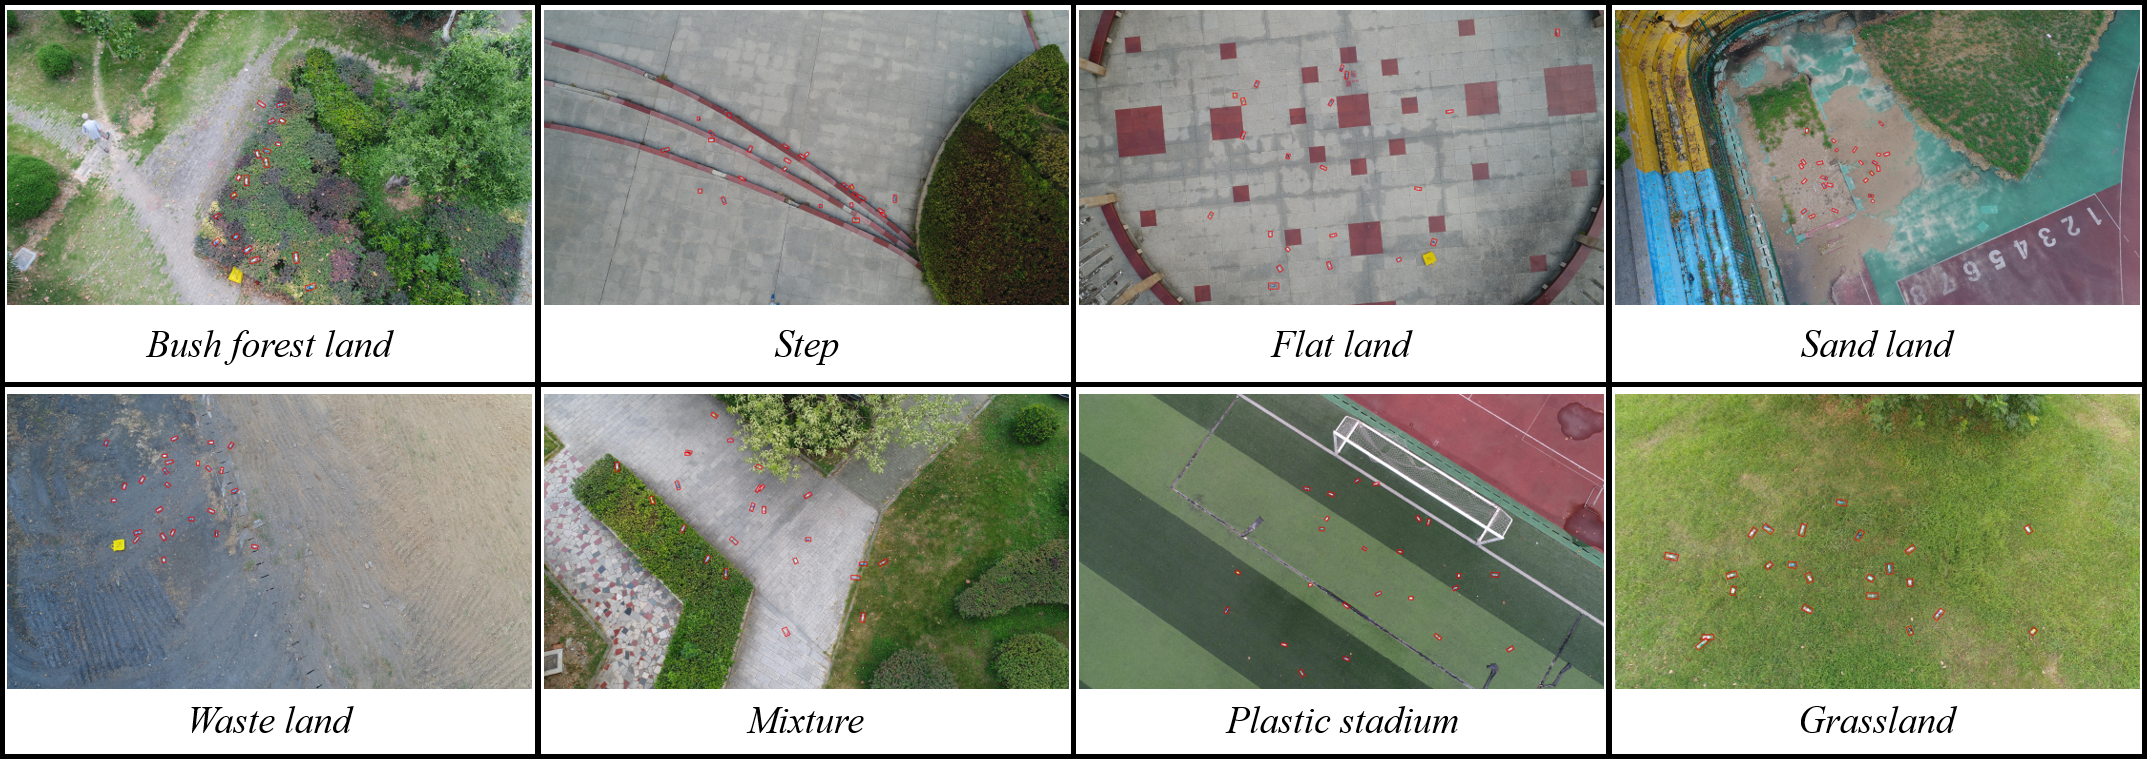
\includegraphics[width=\linewidth]{images/UAV-BD1.png}
	\caption{Samples of annotated images in UAV-BD. We show one full image which size is $ 5472\times 3078 $ per each scene.}
	\label{fig:dataset-original-image}
\end{figure}



\begin{figure}
	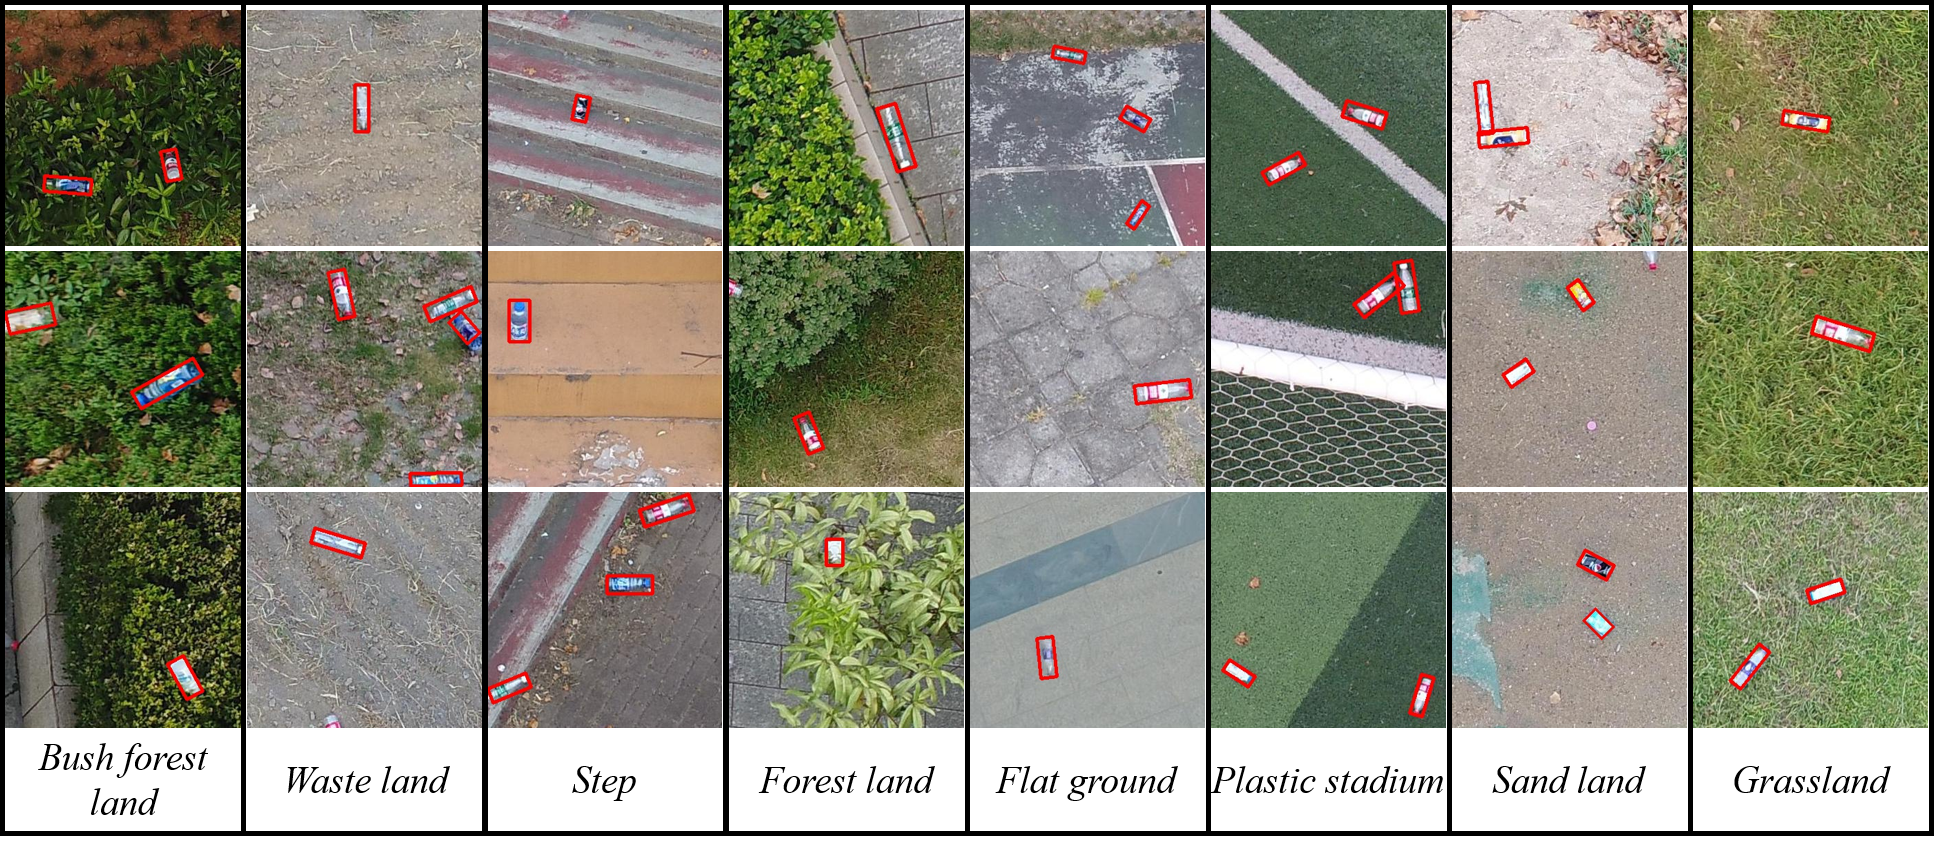
\includegraphics[width=\linewidth]{images/UAV-BD2.png}
	\caption{Sample of annotated images in UAV-BD. We show three images which sizes are $ 342\times 342 $ per each scene.}
	\label{fig:dataset-cut-image}
\end{figure}



%% 2. 数据标注方式
\subsection{Annotation method}
\label{ssec:annotation_method}




We build the UAV-BD for the bottle detection problem by collecting bottle images using UAV. In computer vision field, many visual concepts such as region descriptions, objects, attributes, and relationships, are annotated with horizontal bounding boxes, as show in \cite{DOTA, boundingbox}. A common description of horizontal bounding boxes is $(c_x, c_y, w, h)$ or $ (x_{min}, y_{min}, x_{max}, y_{max}) $, where $(c_x, c_y)$ is the center location of horizontal bounding box, $w, h$ are the width and height and $ (x_{min}, y_{min}) $ is the top left location, $ (x_{max}, y_{max}) $ is the bottom right location\cite{DOTA}. 

Objects with less orientations can be adequately annotated with this method. However, horizontal bounding box cannot accurately or compactly outline oriented instances such as the objects in UAV images. In UAV images, the overlap between two bounding boxes is sometimes very large that some state-of-the-art object detection methods cannot diffetentiate them\cite{DOTA}. At the same time, horizontal bounding box may contain lots of background pixels while annotating the target, especially when objects with large aspect ratios. To solve these problems, we find out a new annotation method for oriented bottles in UAV images.

An option for annotating oriented objects is using the method of arbitrary quadrilatral bounding boxes. This annotation method can be expressed as ${(x_i, y_i), i=1,2,3,4}$, where $(x_i, y_i)$ denotes the position of the oriented bounding boxes' vertices in the image\cite{DOTA}. The vertices are arranged in a clockwise order. But as bottles are rigid with almost no deformation, so we choose a method called $\theta$-based oriented bounding box. This method is often used in text detection benchmarks, expressed as $(c_x, c_y, w, h, \theta)$ where $\theta$ is the angle from the horizontal direction of the horizontal bounding box\cite{DOTA}. The tool for annotating is roLabelImg\footnote{\url{https://github.com/cgvict/roLabelImg.git}}.

\begin{figure}
	\centering
	\subfigure[Normal annotation method using horizontal bounding box]
	{
		\label{angle}
		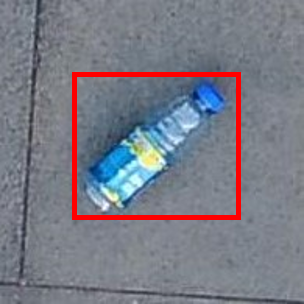
\includegraphics[width=0.45\linewidth]{images/bottle_advantage_2.png}
	}
	\subfigure[Our annotation method using oriented bounding box]
	{
		\label{size}
		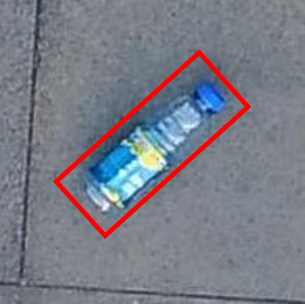
\includegraphics[width=0.45\linewidth]{images/bottle_advantage_1.png}
	}
	\caption{Comparison of traditional bounding box and rotatable bounding box. }
\end{figure}



\subsection{Dataset Splits}

In order to ensure that the distributions of training and testing data approximately match, we randomly select $ 64\% $ of the UAV-BD as the training data, $ 16\% $ as validation data, and $ 20\% $ as the testing data. All the full images and segmented images with ground truth for UAV-BD are publicly available.



%% 3. 数据量统计 
\subsection{Dataset Statistics}
\label{ssec:Dataset_Statistics}
UAV images are usually very large in size compared to conventional image datasets. The size of full image in UAV-BD is $ 5472\times 3078 $, while most images in conventional datasets (e.g. PASCAL VOC and Microsoft COCO) are no more than $ 1000\times 1000 $\cite{RCNNforSmall}. To avoid segmenting the single instances (bottles) into different pieces, we annotate on the full images without segmentation. But we find full image is too large to be trianed for CNN based algorithms. So we segment full images into $ 144 $ small pieces, and the size of piece is $ 342\times 342 $. Note that we abandon the instances at the border. Then we use these small pieces to train CNN based detection model. 


The detialed statistics of the UAV-BD is shown in the Table\ref{statistics}, where $ n_1 $, $ n_2 $, $ n_3 $,  $ n_4 $ are the number of full images, small images, instances in full images, instances in small images for each scene, respectively. And UAV-BD contains about $ 34,791 $ object instances in $ 25,407 $ images. The "Grassland" scene has the largest number of object instances: $ 7,795 $ instances in $ 5,785 $ images. The "Step" scene has the smallest number of instances: $ 2106 $ instances in $ 1,325 $ images.



% Please add the following required packages to your document preamble:
% \usepackage{booktabs}
\begin{table}
	\centering
	\small
	\caption{Images and instances number in UAV-BD}
	\label{statistics}
	\begin{tabular}{@{}ccc|cc@{}}
		\toprule
		Scenes     & $n_1$& $n_2$ & $n_3$ & $n_4$  \\ \midrule
		Bush forest land       & 230  & 4134  & 1812  & 3047  \\
		Waste land     & 379  & 7598  & 4355  & 5800  \\
		Step       & 135  & 2691  & 1325  & 2106  \\
		Forest land    & 285  & 5724  & 3702  & 4891  \\
		Flat land       & 134  & 2803  & 1538  & 2142  \\
		Plastic stadium & 336  & 6807  & 4180  & 4998  \\
		Sand land       & 249  & 5570  & 2704  & 4008  \\
		Grassland       & 456  & 9029  & 5778  & 7787  \\ \midrule
		Total      & 2204 & 44356 & 25394 & 34779 \\ \bottomrule
	\end{tabular}
\end{table}


As bottles usually have rigid body, so we can get some prior information to train the detection model. For example, we can use the distribution of angle, size or ratio as prior information to improve the performance of detection model. For UVA-BD, we plot the distribution of angle, size and ratio respectively, which are illustrated in Fig.\ref{distribution}. From Fig.\ref{angle}, we can see that bottles' angle in the dataset are almost uniform. And most of bottles' size are range from $500 $  pixels to $ 3000 $ pixels while the ratios of bottles are mostly range from $ 1.0 $ to $ 4.0 $, which are shown in Fig.\ref{size} and Fig.\ref{ratio1} . Note that we use these statistics data to design detection models.


\begin{figure}
	\centering
	\subfigure[angle distribution]
	{
		\label{angle}
		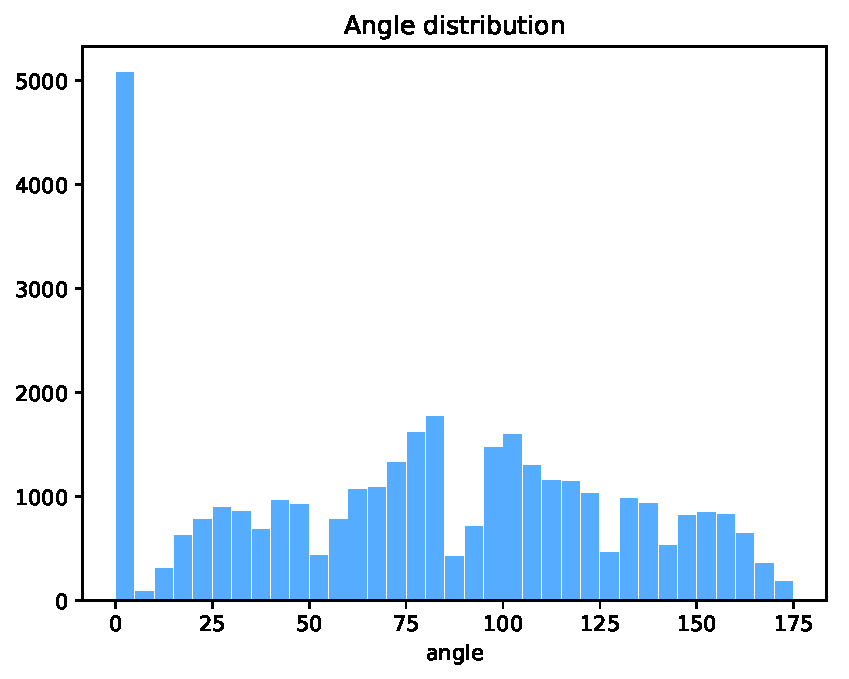
\includegraphics[width=0.45\linewidth]{images/angle_hist.pdf}
	}
	\subfigure[size distribution]
	{
		\label{size}
		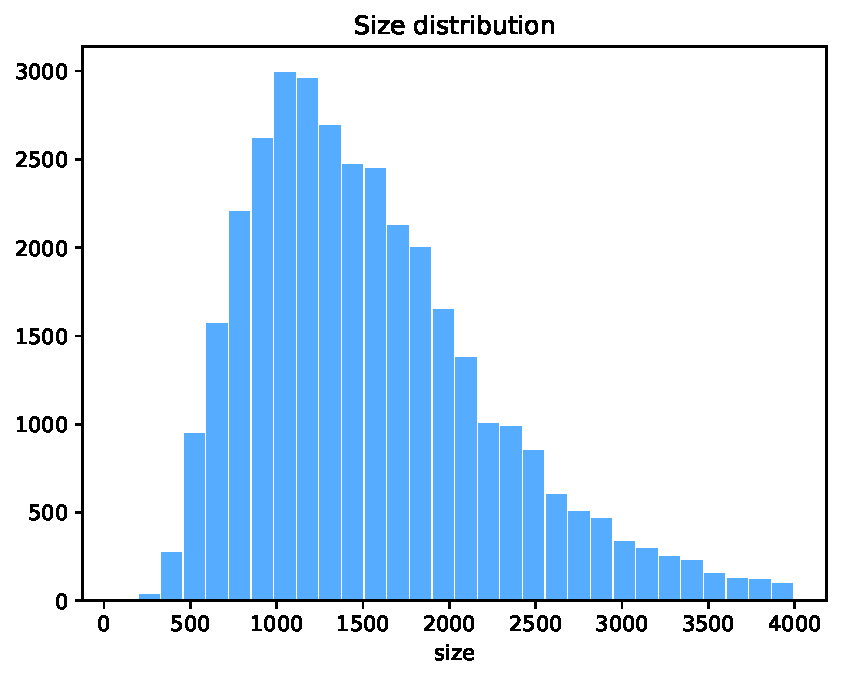
\includegraphics[width=0.45\linewidth]{images/size_hist.pdf}
	}
	\subfigure[ratio distribution]
	{
		\label{ratio1}
		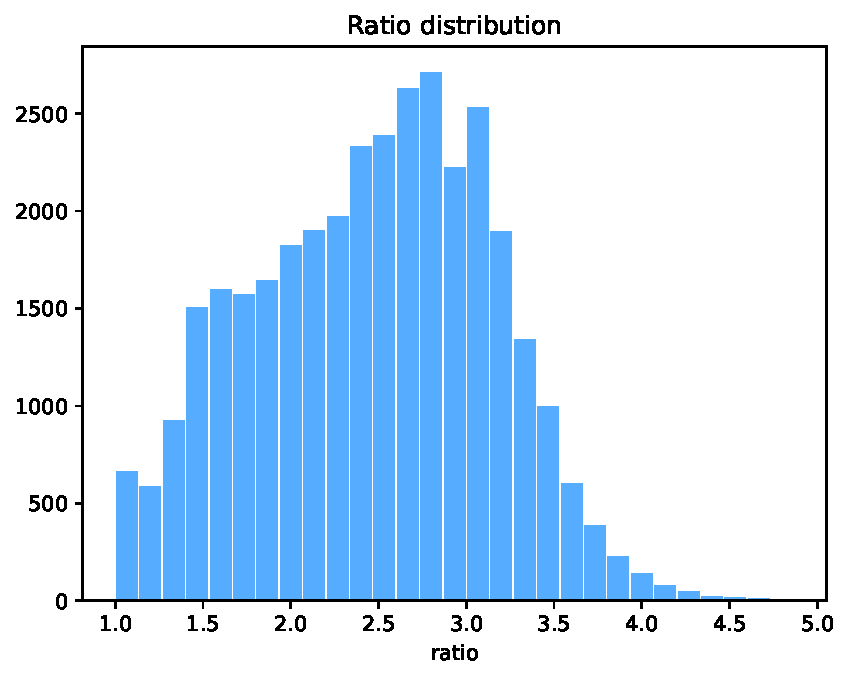
\includegraphics[width=0.45\linewidth]{images/ratio_hist.pdf}
	}
	\caption{The angle, size and ratio distribution of UAV-BD}
	\label{distribution}
\end{figure}


